\documentclass[nofilelist]{cslthse-msc}
% to show a list of used packages at the end of the document, delete the nofilelist option
%\documentclass{cslthse-msc} 
\usepackage[utf8]{inputenc}
\usepackage[english]{babel}
\usepackage{amsmath}
%\usepackage{amsfonts}
%%\usepackage{amssymb}
\usepackage{amsthm}
%\usepackage{makeidx}
\usepackage{graphicx}
\usepackage[titletoc, header, page]{appendix}
\usepackage{transparent}
\usepackage{natbib}
\usepackage{wrapfig}
\usepackage{multirow}
\usepackage{amsmath}

% used to display the used files at the end. Select nofilelist as a package option to disable this
\listfiles % initialize

%\geometry{showframe}
%better like this?
%\student{Flavius Gruian}{Flavius.Gruian@cs.lth.se}
\students{Nick Persson}{dat14npe@student.lu.se}{Filip Karabeleski}{dat14fka.student.lu.se}

\thesisnumber{LU-CS-EX: 2020-XX} % Birger Swahn will provide this number to you, once the thesis is ready for publication
% default is Master. Uncomment the following for "kandidatarbete"/Bachelor's thesis
%\thesistype{Bachelor}{Kandidatarbete}

%\title{Formatting a Master's Thesis}
\title{Keyword Categorization and Emotion Analysis in Voice Calls}

%\onelinetitle
%\twolinestitle
\threelinestitle
%\fourlinestitle

\subtitle{Subtitle WIP}
\company{Telavox AB}
\supervisors
{Sara Lindgren, \href{mailto:Sara.Lindgren@telavox.com}{\texttt{Sara.Lindgren@telavox.com}}}
{Pierre Nugues, \href{mailto:Pierre.Nugues@cs.lth.se}{\texttt{Pierre.Nugues@cs.lth.se.com}}}
\examiner
{Flavius Gruian,\href{mailto:Flavius.Gruian@cs.lth.se}{\texttt{Flavius.Gruian@cs.lth.se}}}

\date{\today}
%\date{January 16, 2015}

\acknowledgements{
If you want to thank people, do it here, on a separate right-hand page. Both the U.S. \textit{acknowledgments} and the British \textit{acknowledgements} spellings are acceptable.

We would like to thank Lennart Andersson for his feedback on this template.

We would also like thank Camilla Lekebjer for her contribution on this template, as well as Magnus Hultin for his popular science summary class and example document.

Thanks also go to the following (former) students for helping with feedback and suggestions on this template: Mikael Persson, Christoffer Lundgren, Mahmoud Nasser.
}

\theabstract{
This document describes the Master's Thesis format for the theses carried out at 
the Department of Computer Science, Lund University. 

Your abstract should capture, in English, the whole thesis with focus on the problem and solution in 150 words. It should be placed on a separate right-hand page, with an additional \textit{1cm} margin on both left and right. Avoid acronyms, footnotes, and references in the abstract if possible.


Leave a \textit{2cm} vertical space after the abstract and provide a few keywords relevant for your report. Use five to six words, of which at most two should be from the title.
}

\keywords{Machine Learning, NLP, Sentiment Analysis, Keyword Extraction, (style, structure)}

%% Only used to display font sizes
\makeatletter
\newcommand\thefontsize[1]{{#1 \f@size pt\par}}
\makeatother
%%%%%%%%%%

\begin{document}
\renewcommand{\bibname}{References}

\makefrontmatter
\chapter{Introduction}

\section{Background}
Natural language processing (NLP) is a field of study mainly in computer science that deals with analyzing human language in a way that computers can understand and process. According to \citet{ntlk2009}, natural language is used for everyday communication by humans, in contrast to artificial languages such as programming languages and mathematical notations. Since natural languages continuously develop as time goes on and its adherence to structures diminish, it is difficult to define explicit rules to follow. 

\subsection{Emotion Recognition}
Emotion has always been a key part of human language, and it therefore comes naturally that teaching a computer to understand emotion in human language is a big part of NLP. Initially, the focus lied in sentiment analysis, a field of study focused on determining the binary polarization of piece of text as either positive or negative. Godtycklig bit om sentiment analysis. 
Emotion recognition is an extension of sentiment analysis that instead of just determining the polarization of text, attributes emotion to it. This process is more challenging than sentiment analysis, as the differences between emotions are subtler than that of just positive and negative. 
Emotion recognition has also been extended to work on different modalities, such as for example visual and auditory input.


Emotion recognition can be applied to data in various modalities, 
such as visual, in the form of facial expressions and body language, audible and text based in the form of dialogues. To o


The LSTM architecture \citep{ntlk2009} is something....

\begin{itemize}
    \item Förklara vad systemet är
    \item Berätta om företaget Telavox
\end{itemize}

\section{Purpose}
\begin{itemize}
    \item Varför behöver problemet lösas, nytta
\end{itemize}
\subsection{Telavox}
Telavox is a telecommunication company that specializes in business-to-business and business-to-customer unified communication as a service. 
\section{Research questions}
The primary aim of this thesis is to investigate whether or not voice call analysis using NLP can be effective enough to be used as a replacement for manual analysis. \\
\textit{What level of precision can be reached with the categorization of keywords from voice calls?}\\
\textit{How well will our algorithm perform compared to other algorithms carrying out the same measurements?}\\
\textit{What level of effectiveness can be reached compared to a human manually analyzing the data?} 

\section{Terminology}
NLP, ML, Speech-to-text och (STT), API. Modality. Kan också kallas för Glossary and Abbreviations
\section{Delimitations}
Delimitations are choices made by the researcher which should be mentioned. They describe the boundaries that you have set for the study.
\section{Contributions}
Potentialen av applications 
\section{Related work}





\chapter{Theory}
\section{Machine Learning}
Machine learning \citep{franoischollet2017learning} is a field of study in artificial intelligence that aims to train a system to solve a problem, rather than to explicitly program it. By being presented with large amounts of data associated with the task at hand, the system algorithmically builds a statistical model that discovers structures in the data and allows the system to identify rules for the problem. 
In \textbf{supervised learning} \citep{100pageBurkov}, which is one of the two main types of tasks in machine learning, the dataset is the collection of labeled examples $\{(\mathbf{x}_i, y_i)\}_{i=1}^N.$ Each element $\mathbf{x}_i$ is a feature vector that contains a value describing the example somehow and $y_i$ is a label, which is either a finite set of classes or a real number. The purpose of supervised learning is to use the dataset to produce a model that takes a feature vector x as input and outputs information that allows deducing the label y for this feature vector.) 
The other main type of tasks in machine learning is \textbf{unsupervised learning}. The dataset for unsupervised learning is $\{ (\mathbf{x}_i)\}_{i=1}^N$ where $\mathbf{x}_i$ is a feature vector. The goal of unsupervised learning is to use the dataset to produce a model that takes a feature vector x as input and outputs either another vector or a value. 



\subsection{Neural Networks and Deep Learning}

Neural networks are machine learning systems loosely inspired by biological neural networks. A neural network is a collection of connected nodes or neurons that was first mentioned in \citet{mcculloch1943}. A neuron \citep{dawson1998ann} is an information-processing unit that receives inputs and produces a single output that can be sent to multiple other neurons. To find the output of a neuron the weighted sum of all inputs is weighted by the weights all connecting to the neuron. This weighted sum is then passed through an activation function to provide the output.

\begin{quote}
RNN gate    
\end{quote}



\begin{quote}
    The learning of the error is the cost function of the network and feeding back is called backpropagation.

\end{quote}

\begin{figure}[htp]
    \centering
    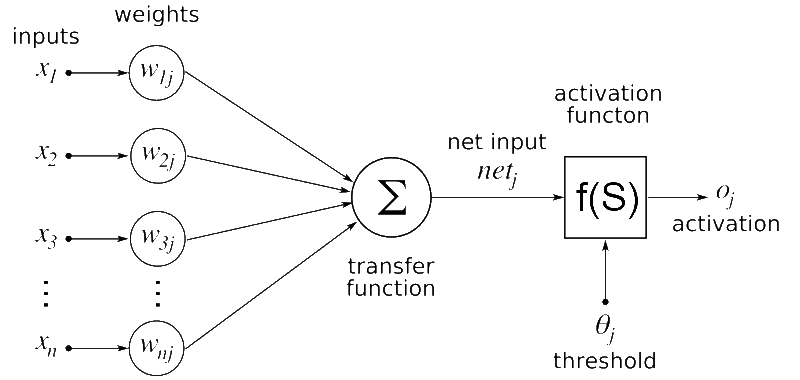
\includegraphics[width=12cm]{msccls/explanatory_images/single_neuron.png}
    \caption{An example of a single neuron}
    \label{fig:neuron}
\end{figure}


\begin{equation}
    g(x_1, x_2, x_3,...,x_n) = g(x) = \sum_{i=1}^n  xi
\end{equation}

Here, $g(x)$ takes the inputs $x_1, x_2, x_3,...,x_n$, while the activation function $f(x)$ defines the output. An example of a well known activation function is ReLU, Rectified linear unit, which has the following function. 

\begin{equation}
y = f(g(x)) =
\begin{cases}
  0, & \text{if}\ x \leq 0 \\
  x, & \text{if}\ x > 0
\end{cases}
\end{equation}





\begin{itemize}
    \item Neurons
    \item Weights and connections 
    \item Backpropagation function
    \item gradient
    \item Deep learning = multiple layers of neural networks
\end{itemize}



\subsection{Gated Recurrent Unit - GRU}
A gated recurrent unit (GRU) is neural network architecture introduced in 2014 by \citet{cho2014learning} and is considered an improvement to the traditional recurrent neural network. Although fairly new it is already a well-established variant of recurrent neural networks. A GRU is quite useful for solving the vanishing gradient problem \citep{hochreiter1998} that might occur in recurrent neural networks. The vanishing gradient problem occurs in machine learning when the gradient progressively decreases, which prevents the adjustments of the weight's values. It has also been shown that GRUs have had better performance on smaller and less frequent datasets \citep{Gruber2020AreGC}.
GRUs is primarily constructed of an update gate, a reset gate and a current memory gate. The update gate regulates the amount of information that is passed along to the next state, while the reset gate on the other hand decides the amount of past information that is going to being disregarded henceforth. 

\begin{quote}
Snacka mer om current memory gate eller ta bort helt
\end{quote}



\subsection{Long Short-Term Memory - LSTM}

\begin{quote}
    Ta bara med ifall vi bestämmer oss att ändra från GRU till LSTM i modellen
    In comparison to GRUs, LSTMs are   

\end{quote}









\section{Word Vectors}
Word vectors are a type of word representation where texts are turned into numbers
\subsection{One-Hot Encoding}
The most basic way of creating a word vector is the one-hot encoding method. This creates a very big and sparse $n \cdot n$ matrix where $n$ is the number of words in the embedding. Each word is then represented by an array filled with zeroes except for one index set to one. For example, the one-hot encoding of the phrase \textit{Why was six afraid of seven} would start with the assignment of values to word:

\begin{center}
    \begin{tabular}{c|c|c|c|c|c}
    
         Why & was & six & afraid & of & seven \\
         \hline
         1 & 2 & 3 & 4 & 5 & 6 \\
    \end{tabular}
\end{center}

This would then be converted into the following matrix:

\begin{center}
    \begin{tabular}{lllllll}
                            & 1 & 2 & 3 & 4 & 5 & 6 \\ \cline{2-7} 
\multicolumn{1}{l|}{Why}    & 1 & 0 & 0 & 0 & 0 & 0 \\
\multicolumn{1}{l|}{was}    & 0 & 1 & 0 & 0 & 0 & 0 \\
\multicolumn{1}{l|}{six}    & 0 & 0 & 1 & 0 & 0 & 0 \\
\multicolumn{1}{l|}{afraid} & 0 & 0 & 0 & 1 & 0 & 0 \\
\multicolumn{1}{l|}{of}     & 0 & 0 & 0 & 0 & 1 & 0 \\
\multicolumn{1}{l|}{seven}  & 0 & 0 & 0 & 0 & 0 & 1
    \end{tabular}
\end{center}

As mentioned, this method is very basic and creates an unnecessarily large matrix that is largely filled up with nothing. If we wanted to represent a vocabulary of 20 000 words, each word would be represented by 19 999 zeroes and a single one. 

The other big issue with it is that no meaning can be extracted from the matrix. If our vocabulary contained the words "cat", "dog" and "hamster", we could easily see that these are all domestic animals but in the space of the one hot vector, "cat" is as close to "dog" as it would be to "airplane". 

\subsection{Word Embedding}
To resolve the two aforementioned problems with one-hot encodings, word embeddings were created, also known as dense word vectors. \citep{neuralnetworkmethods} 
Here, instead of creating a sparse, hardcoded vector with equal distance between words, they are learned from data and packed into a lower-dimensional vector where each dimension contains some relevant data about the word. According to \citet{franoischollet2017learning}, word embeddings that are 256-dimensional, 512-dimensional or 1024-dimensional are common when dealing with very large vocabularies, in contrast to the 20 000-dimensional one that would be created if one were to use one-hot encoding. Additionally, the geometric relationship between words can and should reflect the semantic relationship between those same words. This means that synonyms and words often used together are embedded closer to each other, while words seldom used together are more distant in the embedding. In addition to distance, direction could also be a useful tool to extract meaning from the embedding.\newpage %Temp for formatting, don't forget it's here

\begin{wrapfigure}{r}{0.25\textwidth}
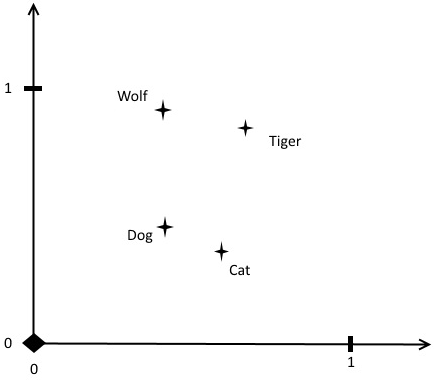
\includegraphics[width=0.9\linewidth]{msccls/explanatory_images/embedding_direction.png} 
\caption{Small example of a word embedding space}
\label{fig:direction}
\end{wrapfigure}


In figure \ref{fig:direction}, the four words \textit{cat}, \textit{dog}, \textit{wolf} and \textit{tiger} are represented on a geometric plane. We can clearly see some of the possible geometric transformations possible by using direction as a tool. For instance, the same vector that takes us from \textit{dog} to \textit{wolf} also takes us from \textit{cat} to \textit{tiger}. This could be interpreted this vector as "converting a domesticated animal to its wildlife equivalent". Another vector will take us both from \textit{cat} to \textit{dog} and from \textit{tiger} to \textit{wolf} which could be interpreted as "converting a feline to a canine". Two meaningful transformation vectors that are common in the real world are "gender" and "plural" vectors. By applying a "female" vector to \textit{king}, \textit{queen} is obtained and the same vector returns \textit{actress} if instead used on \textit{actor}. "Plural", as should seem obvious by now, if used on \textit{actor} will return \textit{actors}. Typically there are thousands of these types of interpretable direction vectors in a large word embedding.


This bit is after the picture, that should be to the right of the last paragraph

\subsection{RoBERTa}

\section{Evaluation}
\subsection{F1-score, precision, accuracy}


\section{Baseline - COSMIC}
\begin{itemize}
    \item Dataset till input måste följa Googles standard som de följer vid speech to text. 
\end{itemize}

\section{Theory}
NLP technique, categorization, ML, supervised/unsupervised,  
Mechanical turks to 
Finns både text och audio på MELD, \citep{zhang2019modeling} visar att text för sig är bättre än ljud men att text+ljud > text
train, dev(validation), test, man testar på dev under development, först på test efter man är klar

\chapter{Implementation}

\section{Datasets}

\subsection{Approach} 
\section{Method}
Google Colab
Word level one hot encoding, kanske relevant, avgör beroende på hur mycket mer vi behöver skriva.
\section{Implementation}
Overfitting \\
Data Augmentation \\
importance of finding the correct data-sets \\
\section{Bibtesting, will be removed}
\citep{emotionlinesdataset} \\
\citep{franoischollet2017learning}\\
\citep{beaver2020towards}
\chapter{Speech-to-text}
Vi antar att det är 2 speakers i samtalet, nämn för- och nackdelar. Ta med i limitations
Vi har endast stöd för engelska pga limits i datamängd, dokumentation. 
Google diarization är i Beta.
Använda kategoriserade ord i Googles STTs speechContexts och därefter använda ML igen för att få högre precision på kategorisering. 
Sample rates 8000 vs 48000 t.ex.

Cased eller uncased? Hur fungerar google speech-to-text med cased/uncased?

\chapter{Keyword Extraction}
\chapter{Emotion Analysis}
6 eller 4 känslor
Sentiment analysis, varför valde vi inte det?


\chapter{Evaluation}

\section{Results}

These are our results

% Please add the following required packages to your document preamble:
% \usepackage{multirow}
\begin{center}
\begin{tabular}{|c|cc|cc|cc|cc|}
\hline
\multirow{2}{*}{Methods} & \multicolumn{2}{c|}{MELD 34}            & \multicolumn{2}{c|}{DailyDialog 45}     & \multicolumn{2}{c|}{IEMOCAP 34}         & \multicolumn{2}{c|}{EmoryNLP 23}        \\ \cline{2-9} 
                         & \multicolumn{1}{c|}{W-Avg F1} & Loss & \multicolumn{1}{c|}{W-Avg F1} & Loss & \multicolumn{1}{c|}{W-Avg F1} & Loss & \multicolumn{1}{c|}{W-Avg F1} & Loss \\ \hline
Cosmic                   & 64.14                         & 2.68 & 60.01                         & 2.94 & 58.77                         & 0.96 & 42.55                         & 2.48 \\ \hline
Vår modell               &                               &      &                               &      &                               &      &                               &      \\ \hline
\end{tabular}
\end{center}


\section{Discussion}
This is the discussion about our results


\chapter{Conclusions}



% Should use consistent formatting when it comes to Names ("FirstName LastName", or "F. LastName")
%\printbibliography
\makebibliography{MyMSc}

\begin{appendices}
\chapter{Dummy Appendix}






% display used packages information unless nofilelist is used in the cslthse-msc package option
\printfilelist

%make sure we're on even page with the pop-sci
\checkoddpage
\ifoddpage
\else
   \newpage
   \thispagestyle{empty}
   \mbox{ }
\fi
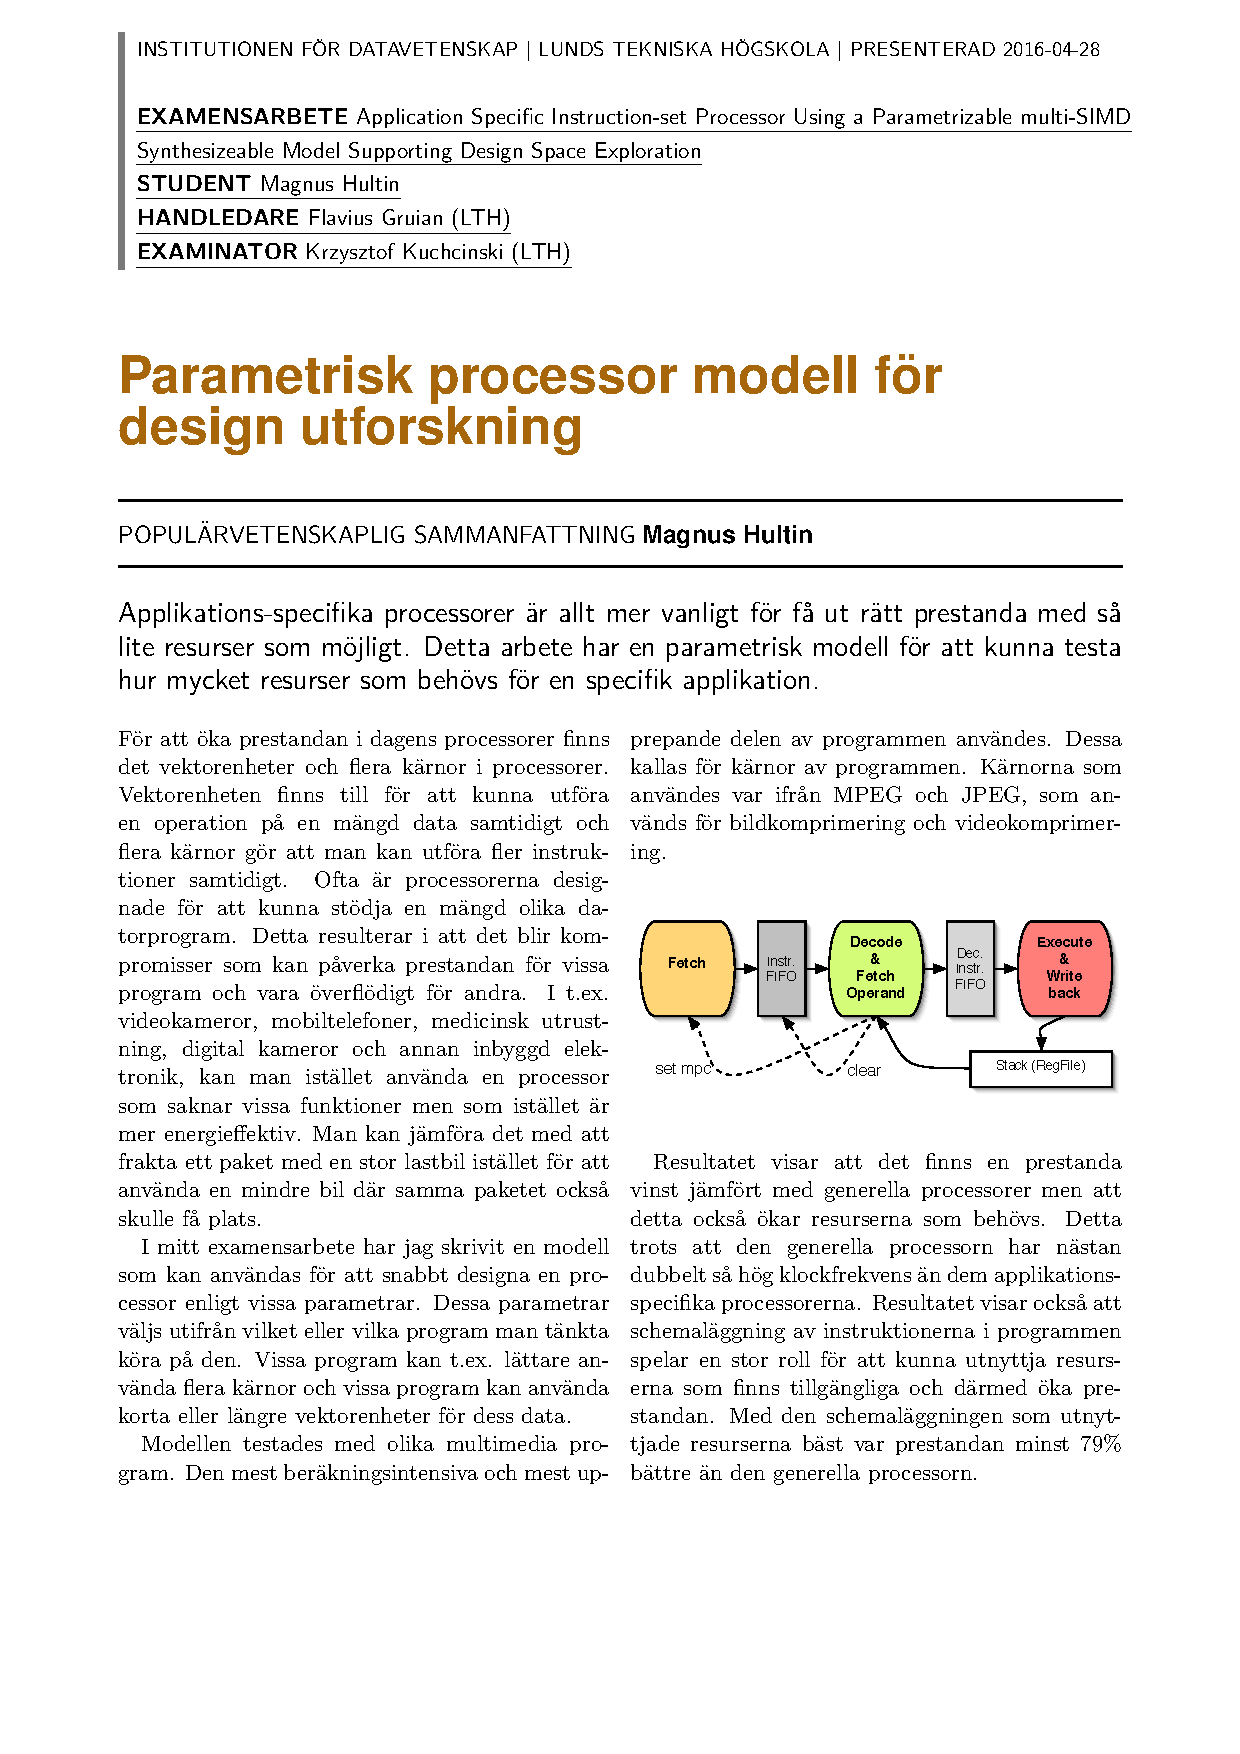
\includepdf[pages={1}]{popsci/popsci.pdf}
\end{appendices}

\end{document}